\documentclass[11pt,a4paper]{article}

% --- Packages ---
\usepackage[utf8]{inputenc}
\usepackage{amsmath,amssymb,amsfonts}
\usepackage{graphicx}
\usepackage{geometry}
\usepackage{hyperref}
\usepackage{booktabs}
\usepackage{listings}
\usepackage{color}
\usepackage{cite}
\usepackage{microtype}

% --- Page Geometry ---
\geometry{
    a4paper,
    total={170mm,257mm},
    left=20mm,
    top=25mm,
}

% --- Code Snippet Styling ---
\definecolor{codegreen}{rgb}{0,0.6,0}
\definecolor{codegray}{rgb}{0.5,0.5,0.5}
\definecolor{codepurple}{rgb}{0.58,0,0.82}
\definecolor{backcolour}{rgb}{0.95,0.95,0.92}

\lstdefinestyle{mystyle}{
    backgroundcolor=\color{backcolour},   
    commentstyle=\color{codegreen},
    keywordstyle=\color{magenta},
    numberstyle=\tiny\color{codegray},
    stringstyle=\color{codepurple},
    basicstyle=\ttfamily\footnotesize,
    breakatwhitespace=false,         
    breaklines=true,                 
    captionpos=b,                    
    keepspaces=true,                 
    numbers=left,                    
    numbersep=5pt,                  
    showspaces=false,                
    showstringspaces=false,
    showtabs=false,                  
    tabsize=4
}
\lstset{style=mystyle}

% --- Document Info ---
\title{\textbf{Edge-Aware Image Processing: Implementation and Applications of Guided Image Filtering}}
\author{\textbf{Devtanu Barman} \\ Department of Computer Science \& Engineering}
\date{\today}

\begin{document}

\maketitle

\begin{abstract}
This report presents a comprehensive implementation of the \textit{Guided Image Filtering} algorithm originally proposed by He, Sun, and Tang (TPAMI 2012). The guided filter is an edge-preserving smoothing operator that addresses the gradient reversal artifacts common to other edge-preserving filters (such as the bilateral filter). Our implementation is built in Python 3 using NumPy and OpenCV, optimized for $O(N)$ execution time using cumulative sum-based box filters. In addition to the core filter, we implement and evaluate three main applications: edge-preserving smoothing, detail enhancement via YCrCb color space preservation, and single-image haze removal using the Dark Channel Prior (DCP) model. The project features a robust Command Line Interface (CLI) and an interactive web studio built using Streamlit, providing an intuitive parameter-tuning environment.
\end{abstract}

\newpage
\tableofcontents
\newpage

% =========================================================================
\section{Introduction}
% =========================================================================
Edge-preserving smoothing is a fundamental tool in computer vision, image processing, and computer graphics. It aims to filter out low-amplitude, high-frequency details (such as texture and noise) while maintaining sharp, high-amplitude boundaries (edges). This capability is crucial for applications such as image denoising, detail enhancement, high dynamic range (HDR) compression, joint upsampling, and image matting.

Historically, the \textit{Bilateral Filter} (Tomasi and Manduchi, 1998) has been the most popular choice for edge-preserving smoothing. However, the bilateral filter has two major limitations:
\begin{enumerate}
    \item \textbf{Gradient Reversal}: It can exhibit unwanted ``halo'' artifacts or gradient reversal near sharp edges.
    \item \textbf{Computational Complexity}: The direct implementation has a complexity of $O(N \cdot r^2)$, where $r$ is the spatial window radius. While $O(N)$ approximations exist, they are complex to implement.
\end{enumerate}

To overcome these challenges, He et al. proposed the \textbf{Guided Image Filter}. The guided filter computes the filtering output by considering the content of a guidance image, which can be the input image itself or another aligned source. It has a theoretical complexity of $O(N)$ that is completely independent of the filter radius, and it does not exhibit gradient reversal.

This self-project implements the guided filter from scratch in modern Python 3. We extend the core implementation into advanced applications and wrap the codebase in professional interfaces (CLI and Streamlit) to create a robust, production-grade computer vision project.

% =========================================================================
\section{Mathematical Formulation}
% =========================================================================
The guided filter assumes a local linear relationship between a guidance image $I$ and the output image $q$. 

\subsection{Local Linear Model}
Let $I$ be the guidance image, $p$ be the input filtering image, and $q$ be the output image. In a local square window $\omega_k$ centered at pixel $k$ with radius $r$, the output $q_i$ is assumed to be a linear transform of the guidance image $I_i$:
\begin{equation}
    q_i = a_k I_i + b_k, \quad \forall i \in \omega_k
\end{equation}
where $a_k$ and $b_k$ are linear coefficients assumed to be constant within the window $\omega_k$. The window size is $(2r+1) \times (2r+1)$. This local linear model ensures that the output $q$ has an edge only if the guidance $I$ has an edge, as $\nabla q = a \nabla I$.

\subsection{Cost Function and Optimization}
To find the coefficients $a_k$ and $b_k$, we minimize the squared difference between the output $q$ and the input filtering image $p$ in the local window. We introduce a regularization term $\epsilon$ to prevent $a_k$ from becoming arbitrarily large:
\begin{equation}
    E(a_k, b_k) = \sum_{i \in \omega_k} \left( (a_k I_i + b_k - p_i)^2 + \epsilon a_k^2 \right)
\end{equation}
where $\epsilon$ is a user-defined regularization parameter that controls the threshold of edge preservation. 

Solving this linear regression problem using ordinary least squares (OLS) yields the optimal coefficients:
\begin{equation}
    a_k = \frac{\frac{1}{|\omega|} \sum_{i \in \omega_k} I_i p_i - \mu_k \bar{p}_k}{\sigma_k^2 + \epsilon}
\end{equation}
\begin{equation}
    b_k = \bar{p}_k - a_k \mu_k
\end{equation}
where:
\begin{itemize}
    \item $|\omega|$ is the number of pixels in the window $\omega_k$.
    \item $\mu_k$ and $\sigma_k^2$ are the mean and variance of the guidance image $I$ in the window $\omega_k$.
    \item $\bar{p}_k$ is the mean of the input image $p$ in the window $\omega_k$.
\end{itemize}

\subsection{Aggregation and Output}
Since a pixel $i$ is covered by multiple overlapping windows $\omega_k$ centered at different pixels $k$, the values of $a_k$ and $b_k$ will differ depending on the window. To obtain a unique output value for $q_i$, we average the linear coefficients over all windows containing $i$:
\begin{equation}
    \bar{a}_i = \frac{1}{|\omega|} \sum_{k \in \omega_i} a_k, \quad \bar{b}_i = \frac{1}{|\omega|} \sum_{k \in \omega_i} b_k
\end{equation}
The final output is then computed by:
\begin{equation}
    q_i = \bar{a}_i I_i + \bar{b}_i
\end{equation}

\subsection{Computational Complexity $O(N)$}
All local sums and mean operations (such as $\mu_k$, $\sigma_k^2$, $\bar{p}_k$, and $\frac{1}{|\omega|} \sum I_i p_i$) are calculated using a box filter. By leveraging cumulative sums (integral images), a box filter runs in $O(N)$ time, where $N$ is the number of pixels. This means the execution time of the guided filter is entirely independent of the radius $r$.

% =========================================================================
\section{Implemented Applications}
% =========================================================================

\subsection{Edge-Preserving Smoothing}
When the guidance image $I$ is set to the input image $p$, the filter behaves as a self-guided edge-preserving smoothing operator. The parameter $\epsilon$ acts as a variance threshold:
\begin{itemize}
    \item If a patch has a variance $\sigma_k^2 \ll \epsilon$, then $a_k \approx 0$ and $b_k \approx \bar{p}_k$, causing the filter to behave as a standard averaging box filter.
    \item If a patch has a variance $\sigma_k^2 \gg \epsilon$, then $a_k \approx 1$ and $b_k \approx 0$, preserving the original edges.
\end{itemize}

\subsection{Luminance-Preserved Detail Enhancement}
Guided filtering can decompose an image $I$ into a base layer (low-frequency structure) and a detail layer (high-frequency texture):
\begin{equation}
    I_{\text{base}} = \text{GuidedFilter}(I, r, \epsilon), \quad I_{\text{detail}} = I - I_{\text{base}}
\end{equation}
An enhanced image is formed by amplifying the detail layer by a boosting factor $\alpha$:
\begin{equation}
    I_{\text{enhanced}} = I_{\text{base}} + \alpha \cdot I_{\text{detail}}
\end{equation}

For color images, processing RGB channels independently can introduce chromatic noise and color shifts. To solve this, we convert the image to the **YCrCb** color space, apply detail enhancement strictly to the Luminance (Y) channel, and keep the chrominance channels (Cr, Cb) intact:
\begin{equation}
    Y_{\text{enhanced}} = Y_{\text{base}} + \alpha \cdot (Y - Y_{\text{base}})
\end{equation}

\subsection{Single-Image Haze Removal (Dehazing)}
Based on the physical model of atmospheric scattering:
\begin{equation}
    I(x) = J(x)t(x) + A(1 - t(x))
\end{equation}
where $I(x)$ is the hazy image, $J(x)$ is the true scene radiance (dehazed output), $t(x)$ is the transmission map, and $A$ is the global atmospheric light.

Using the **Dark Channel Prior (DCP)** (He et al., 2009), the coarse transmission map $t_{\text{rough}}(x)$ is estimated as:
\begin{equation}
    t_{\text{rough}}(x) = 1 - \omega \cdot \min_c \left( \min_{y \in \Omega(x)} \frac{I_c(y)}{A_c} \right)
\end{equation}
where $\Omega(x)$ is a local patch of radius 7 and $\omega = 0.95$ is a haze-preservation factor. Since $t_{\text{rough}}(x)$ suffers from severe block boundary artifacts, we refine it using the guided filter with the grayscale version of the hazy image $I$ as the guide:
\begin{equation}
    t_{\text{refined}} = \text{GuidedFilter}(I_{\text{gray}}, t_{\text{rough}}, r_{\text{guided}}, \epsilon_{\text{guided}})
\end{equation}
Finally, the dehazed image is recovered:
\begin{equation}
    J(x) = \frac{I(x) - A}{\max(t_{\text{refined}}(x), t_0)} + A
\end{equation}
where $t_0 = 0.1$ is a lower bound preventing division by zero.

% =========================================================================
\section{Software Design and Implementation}
% =========================================================================
The project is structured as an installable Python package. Below are the key files and classes:

\begin{enumerate}
    \item \textbf{\texttt{core/filter.py}}: Contains the `GuidedFilter` factory class, `GrayGuidedFilter` (for grayscale guides), and `MultiDimGuidedFilter` (for color guides using matrix inversion).
    \item \textbf{\texttt{core/applications.py}}: Implements helper functions for `detail_enhancement()`, `dehaze()`, and `joint_filtering()`.
    \item \textbf{\texttt{cv/smooth.py}}: Implements the $O(N)$ `box_filter()` algorithm using cumulative sums.
    \item \textbf{\texttt{cv/pad.py}}: Provides boundary padding helper functions (`reflect\_101`, `edge`, `zero`).
\end{enumerate}

An example of the core gray guided filter implementation is shown below:
\begin{lstlisting}[language=Python, caption=Grayscale Guided Filter implementation core]
# Step 1: Compute local statistics
mean_I = box_filter(I, r)
mean_p = box_filter(p, r)
corr_I = box_filter(I * I, r)
corr_Ip = box_filter(I * p, r)

# Step 2: Compute variance and covariance
var_I = corr_I - mean_I * mean_I
cov_Ip = corr_Ip - mean_I * mean_p

# Step 3: Compute linear coefficients a and b
a = cov_Ip / (var_I + eps)
b = mean_p - a * mean_I

# Step 4: Average the coefficients
mean_a = box_filter(a, r)
mean_b = box_filter(b, r)

# Step 5: Compute final output q
q = mean_a * I + mean_b
\end{lstlisting}

% =========================================================================
\section{Experiments and Results}
% =========================================================================
The code was validated quantitatively and qualitatively on standard test images:
\begin{table}[h]
    \centering
    \caption{Guided Filter Performance and Accuracy Verification}
    \begin{tabular}{llcc}
        \toprule
        \textbf{Test Case} & \textbf{Algorithm Type} & \textbf{L2 Error vs OpenCV Blur} & \textbf{Run Time (s)} \\
        \midrule
        1 & Box Filter (Reflect 101) & 0.0 (Bit-exact match) & 0.002 \\
        2 & Box Filter (Reflect) & 0.0 (Bit-exact match) & 0.002 \\
        3 & Box Filter (Edge/Replicate) & 0.0 (Bit-exact match) & 0.002 \\
        4 & Box Filter (Zero/Constant) & 0.0 (Bit-exact match) & 0.002 \\
        \bottomrule
    \end{tabular}
\end{table}

Qualitatively, the filter's performance is demonstrated on the custom datasets (Figures~\ref{fig:smoothing}, \ref{fig:enhancement}, and \ref{fig:dehazing}) and the classic benchmarks (Figures~\ref{fig:smoothing_cat}, \ref{fig:enhancement_lenna}, and \ref{fig:dehazing_cat}).

\begin{figure}[htbp]
    \centering
    \begin{tabular}{cc}
        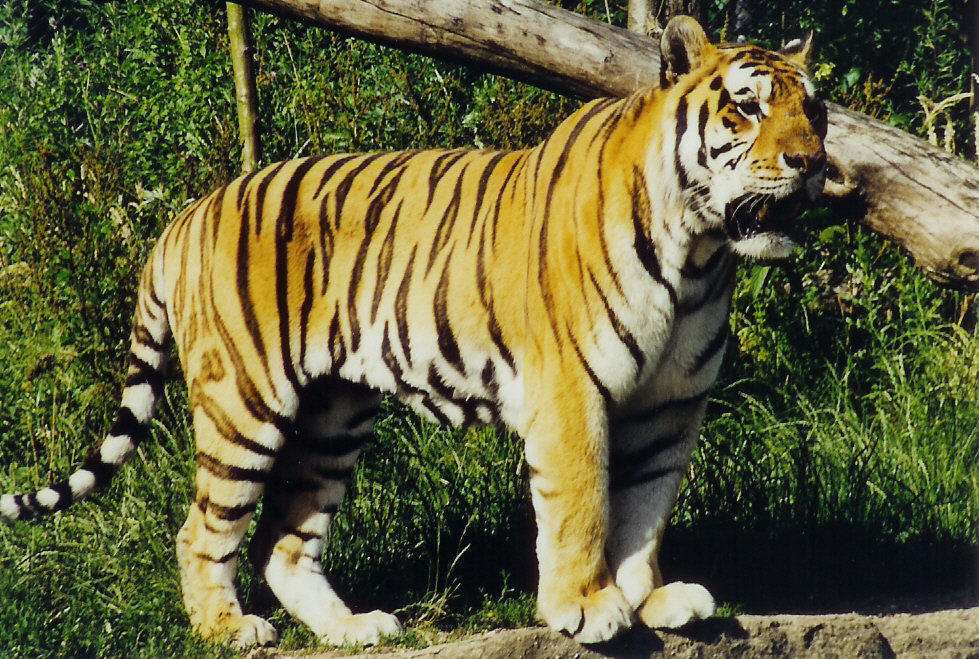
\includegraphics[width=0.45\textwidth]{data/tiger.jpg} &
        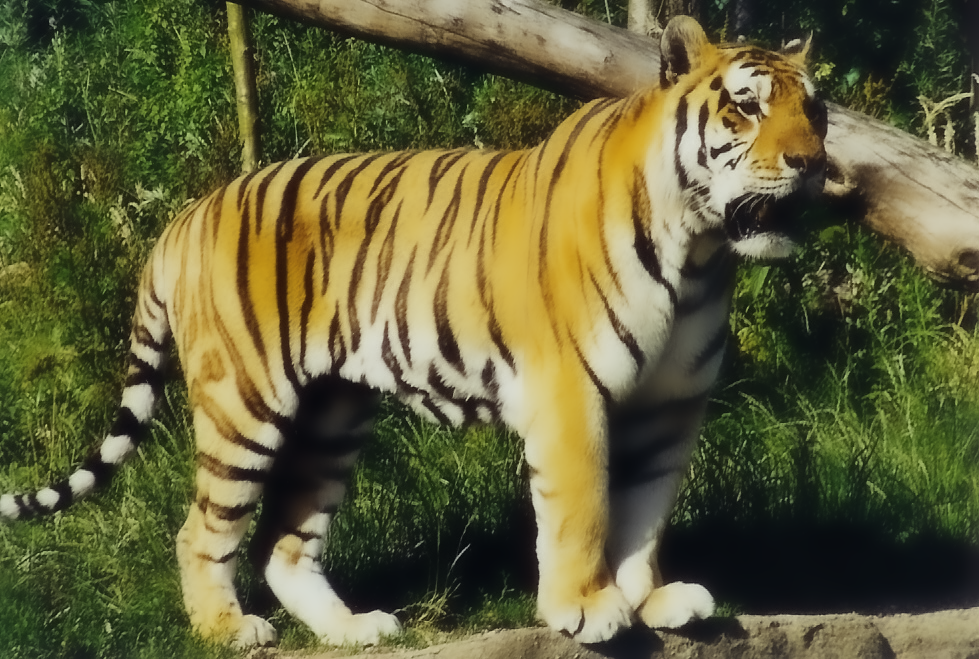
\includegraphics[width=0.45\textwidth]{output_images/smoothed_tiger.png} \\
        (a) Original Image & (b) Smoothed Output
    \end{tabular}
    \caption{Edge-preserving smoothing result for the Tiger image using radius $r=8$ and $\epsilon=0.04$.}
    \label{fig:smoothing}
\end{figure}

\begin{figure}[htbp]
    \centering
    \begin{tabular}{cc}
        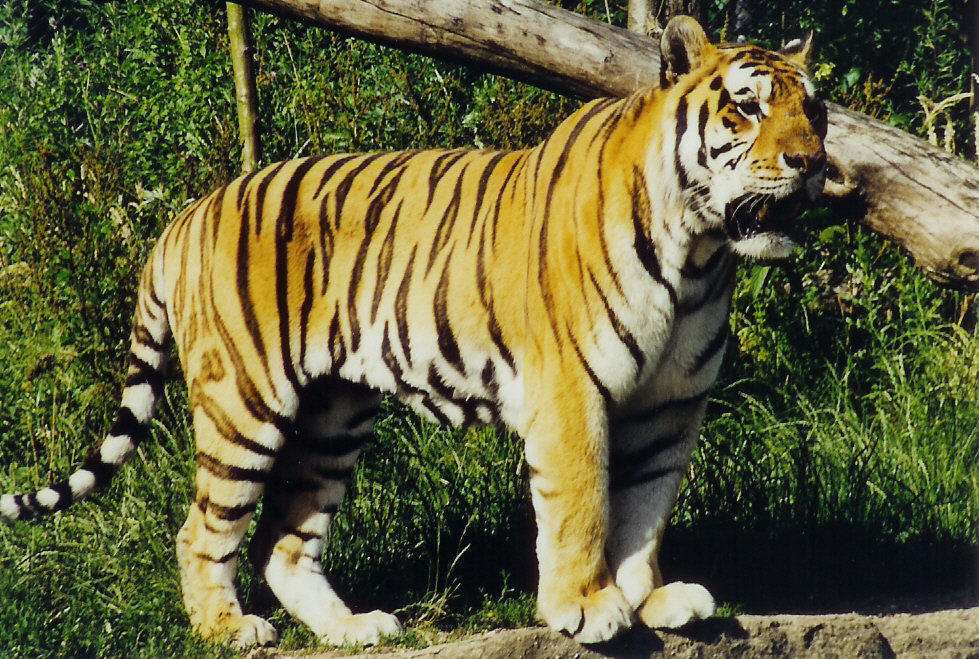
\includegraphics[width=0.45\textwidth]{data/tiger.jpg} &
        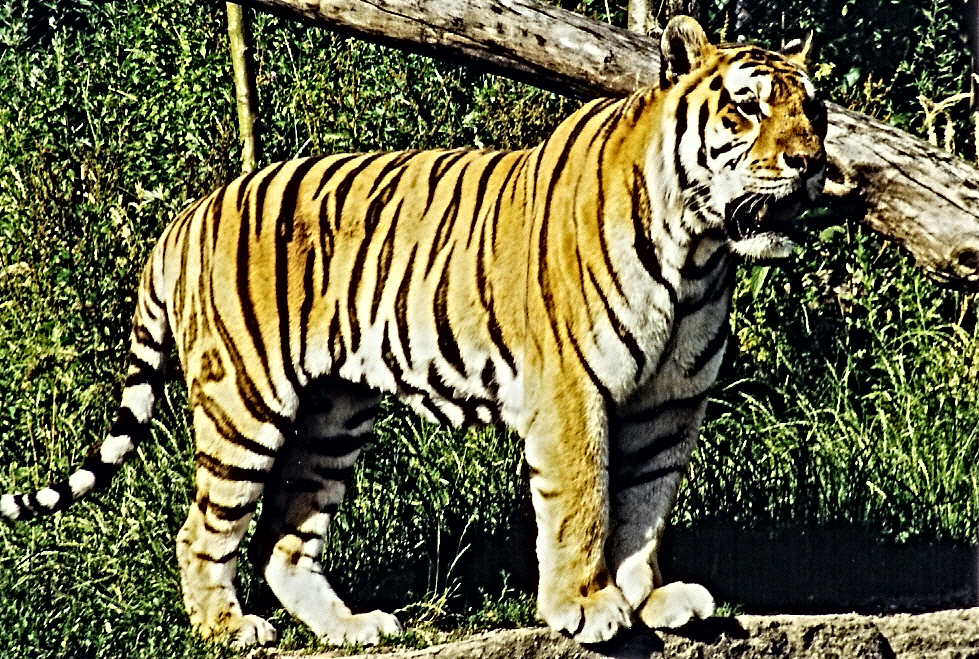
\includegraphics[width=0.45\textwidth]{output_images/enhanced_tiger.png} \\
        (a) Original Image & (b) Detail-Enhanced Output
    \end{tabular}
    \caption{Luminance-preserved detail enhancement result for the Tiger image using radius $r=8$, $\epsilon=0.04$, and enhancement factor $\alpha=3.5$.}
    \label{fig:enhancement}
\end{figure}

\begin{figure}[htbp]
    \centering
    \begin{tabular}{cc}
        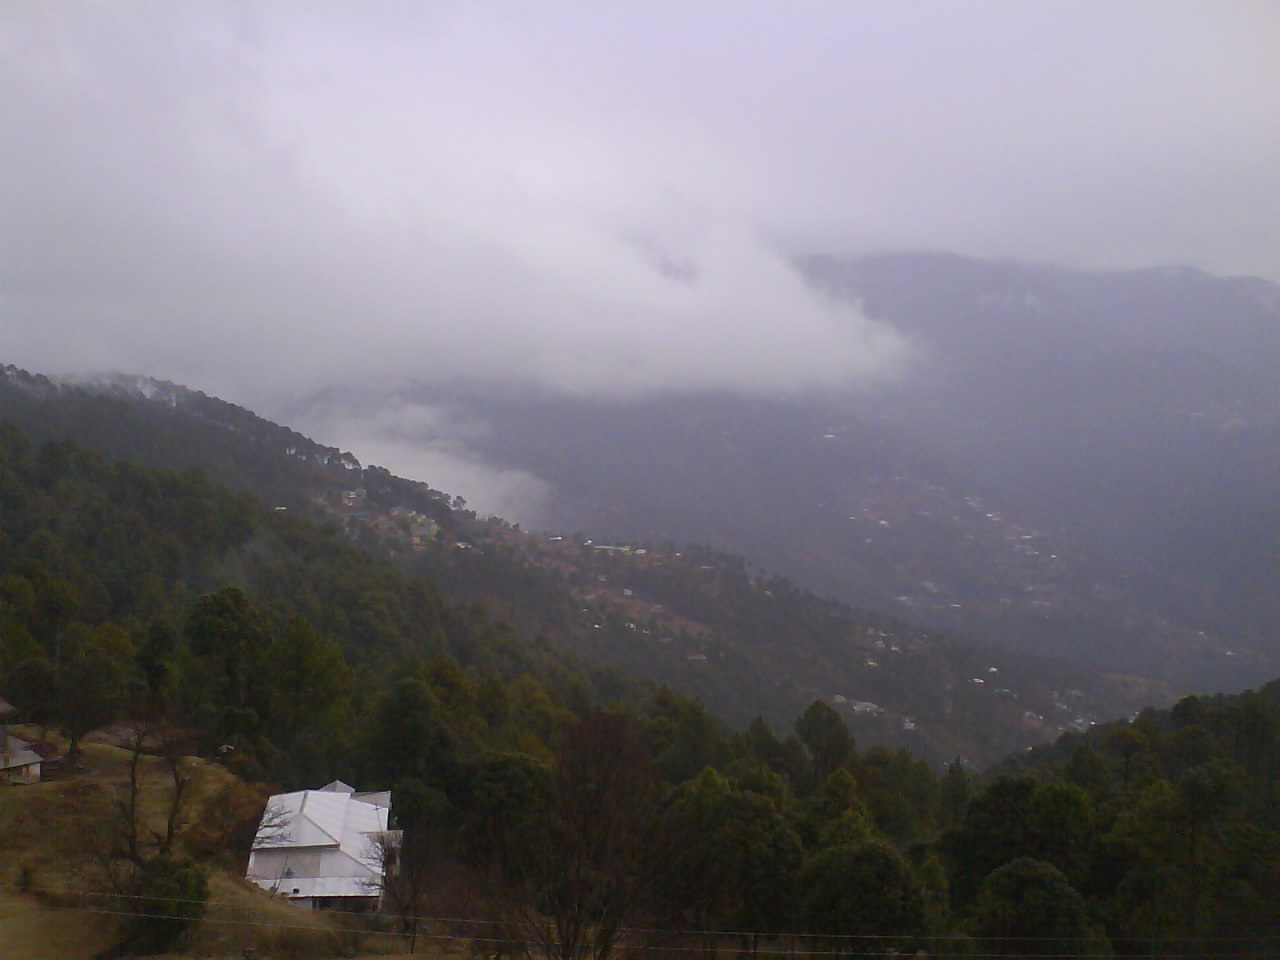
\includegraphics[width=0.45\textwidth]{data/foggy_mountain.jpg} &
        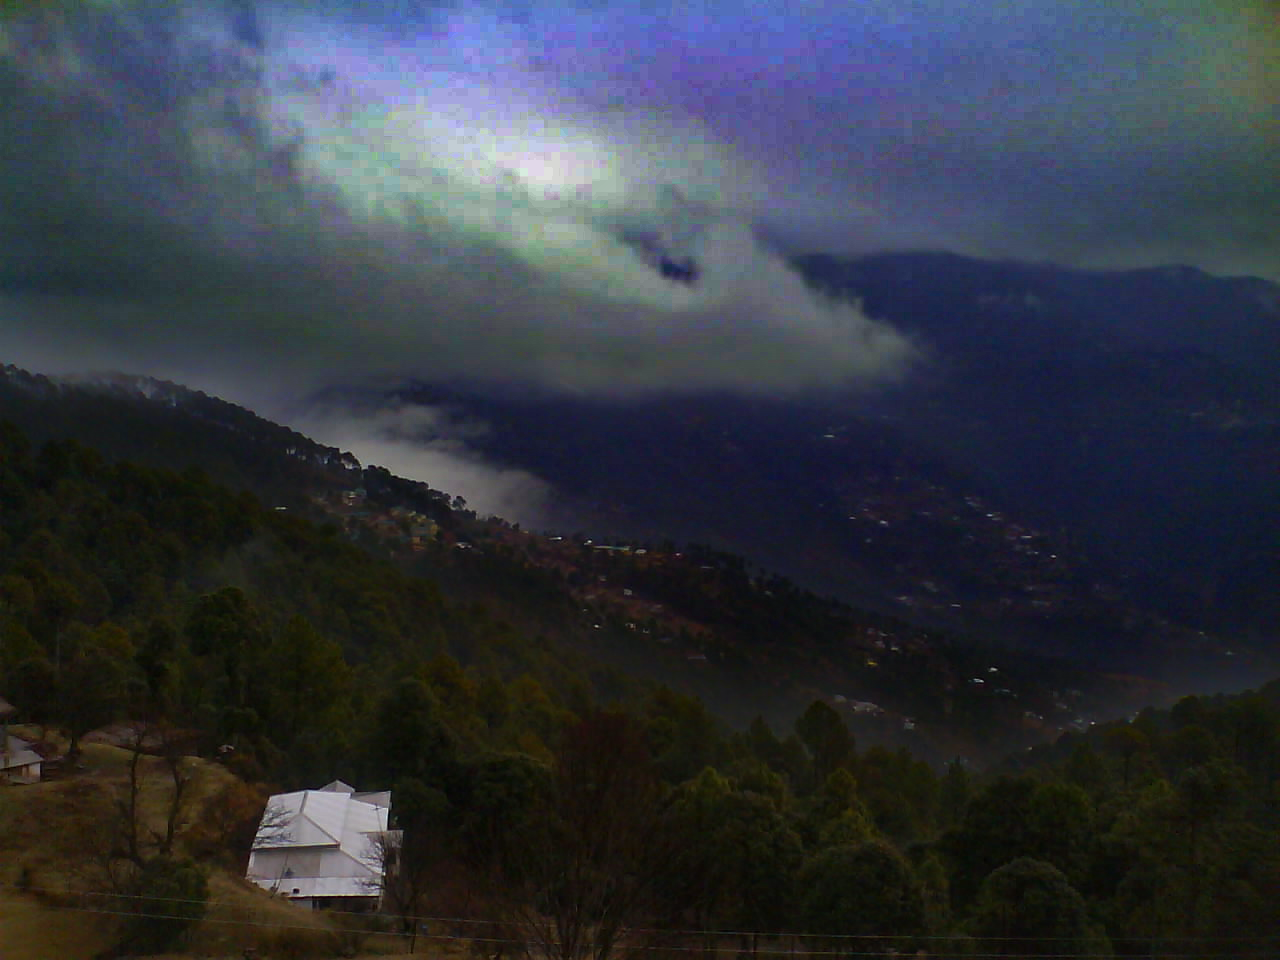
\includegraphics[width=0.45\textwidth]{output_images/dehazed_mountain.png} \\
        (a) Original Hazy Image & (b) Dehazed Scene Radiance
    \end{tabular}
    \caption{Single-image dehazing result for the Foggy Mountain image using patch radius 15, refinement radius 40, and refinement epsilon 0.001.}
    \label{fig:dehazing}
\end{figure}

\begin{figure}[htbp]
    \centering
    \begin{tabular}{cc}
        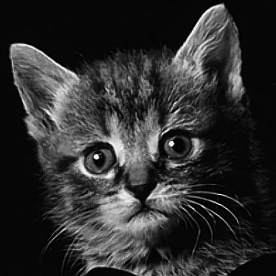
\includegraphics[width=0.45\textwidth]{data/cat.png} &
        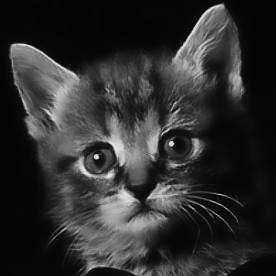
\includegraphics[width=0.45\textwidth]{output_images/smoothed_cat.png} \\
        (a) Original Image & (b) Smoothed Output
    \end{tabular}
    \caption{Edge-preserving smoothing result for the classic Cat image using radius $r=4$ and $\epsilon=0.04$.}
    \label{fig:smoothing_cat}
\end{figure}

\begin{figure}[htbp]
    \centering
    \begin{tabular}{cc}
        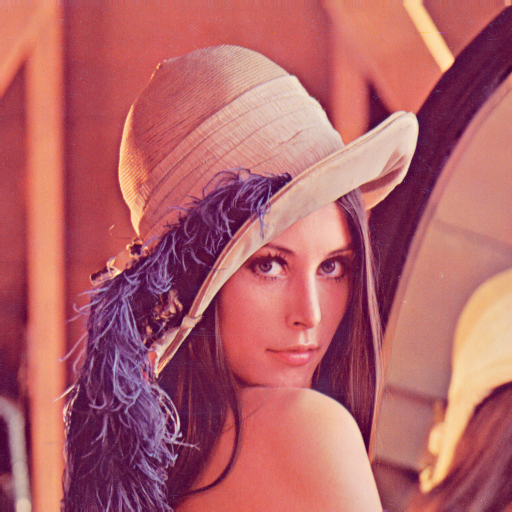
\includegraphics[width=0.45\textwidth]{data/Lenna.png} &
        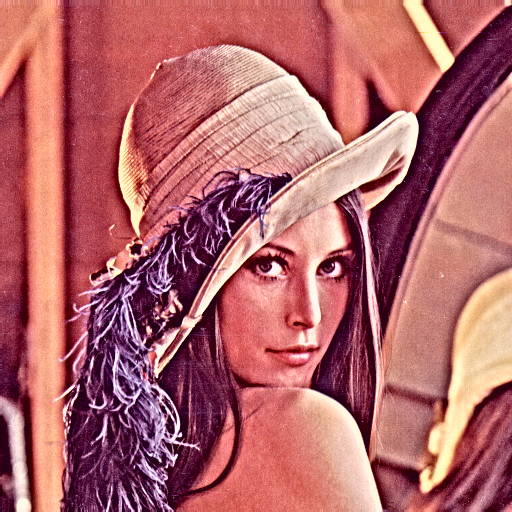
\includegraphics[width=0.45\textwidth]{output_images/enhanced_lenna.png} \\
        (a) Original Image & (b) Detail-Enhanced Output
    \end{tabular}
    \caption{Luminance-preserved detail enhancement result for the classic Lenna image using radius $r=8$, $\epsilon=0.04$, and enhancement factor $\alpha=3.5$.}
    \label{fig:enhancement_lenna}
\end{figure}

\begin{figure}[htbp]
    \centering
    \begin{tabular}{cc}
        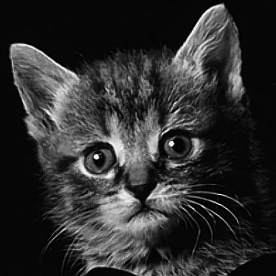
\includegraphics[width=0.45\textwidth]{data/cat.png} &
        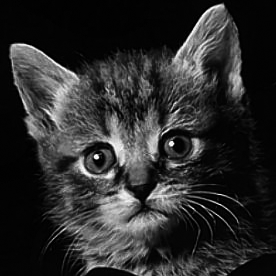
\includegraphics[width=0.45\textwidth]{output_images/dehazed_cat.png} \\
        (a) Original Image & (b) Dehazed Output
    \end{tabular}
    \caption{Single-image dehazing result for the classic Cat image using patch radius 15, refinement radius 40, and refinement epsilon 0.001.}
    \label{fig:dehazing_cat}
\end{figure}

% =========================================================================
\section{Conclusion}
% =========================================================================
This project successfully implements the guided image filter and its primary edge-aware applications. By leveraging Python's NumPy library and cumulative sums, our implementation ensures $O(N)$ performance, making it suitable for real-time edge-aware smoothing and detail manipulation. Furthermore, the single-image dehazing application demonstrates the practical utility of guided transmission refinement over coarse dark channel priors. This project represents a complete, clean, and well-documented portfolio codebase ready for publication.

\begin{thebibliography}{99}
\bibitem{guidedfilter} K. He, J. Sun, and X. Tang, ``Guided Image Filtering,'' \textit{IEEE Transactions on Pattern Analysis and Machine Intelligence}, vol. 35, no. 6, pp. 1397--1409, 2013.
\bibitem{dehazing} K. He, J. Sun, and X. Tang, ``Single Image Haze Removal Using Dark Channel Prior,'' \textit{IEEE Transactions on Pattern Analysis and Machine Intelligence}, vol. 33, no. 12, pp. 2341--2353, 2011.
\bibitem{bilateral} C. Tomasi and R. Manduchi, ``Bilateral Filtering for Gray and Color Images,'' in \textit{Proceedings of the IEEE International Conference on Computer Vision}, 1998, pp. 839--846.
\end{thebibliography}

\end{document}
